\documentclass[14pt,a4paper]{report}  %紙張設定
\usepackage{xeCJK}%中文字體模組
%\setCJKmainfont{標楷體} % 在 windows 設定中文字體 
\setCJKmainfont{MoeStandardKai.ttf}
%\newfontfamily\sectionef{Times New Roman} % 在 windows 設定英文字體
\newfontfamily\sectionef{Nimbus Roman}
\usepackage{enumerate}
\usepackage{amsmath,amssymb}%數學公式、符號
\usepackage{amsfonts} %數學簍空的英文字
\usepackage{graphicx, subfigure}%圖形
\usepackage{fontawesome5} %引用icon
\usepackage{type1cm} %調整字體絕對大小
\usepackage{textpos} %設定文字絕對位置
\usepackage[top=2.5truecm,bottom=2.5truecm,
left=3truecm,right=2.5truecm]{geometry}
\usepackage{titlesec} %目錄標題設定模組
\usepackage{titletoc} %目錄內容設定模組
\usepackage{textcomp} %表格設定模組
\usepackage{multirow} %合併行
%\usepackage{multicol} %合併欄
\usepackage{CJK} %中文模組
\usepackage{CJKnumb} %中文數字模組
\usepackage{wallpaper} %浮水印
\usepackage{listings} %引用程式碼
\usepackage{hyperref} %引用url連結
\usepackage{setspace}
\usepackage{lscape}%設定橫式
\usepackage{url}
\lstset{language=Python, %設定語言
		basicstyle=\fontsize{10pt}{2pt}\selectfont, %設定程式內文字體大小
		frame=lines,	%設定程式框架為線
}
%\usepackage{subcaption}%副圖標
\graphicspath{{./../images/}} %圖片預設讀取路徑
\usepackage{indentfirst} %設定開頭縮排模組
\renewcommand{\figurename}{\Large 圖.} %更改圖片標題名稱
\renewcommand{\tablename}{\Large 表.}
\renewcommand{\lstlistingname}{\Large 程式.} %設定程式標示名稱
\hoffset=-5mm %調整左右邊界
\voffset=-8mm %調整上下邊界
\setlength{\parindent}{3em}%設定首行行距縮排
\usepackage{appendix} %附錄
\usepackage{diagbox}%引用表格
\usepackage{multirow}%表格置中
%\usepackage{number line}
%=------------------更改標題內容----------------------=%
\titleformat{\chapter}[hang]{\center\sectionef\fontsize{20pt}{1pt}\bfseries}{\LARGE 第\CJKnumber{\thechapter}章}{1em}{}[]
\titleformat{\section}[hang]{\sectionef\fontsize{18pt}{2.5pt}\bfseries}{{\thesection}}{0.5em}{}[]
\titleformat{\subsection}[hang]{\sectionef\fontsize{18pt}{2.5pt}\bfseries}{{\thesubsection}}{1em}{}[]
%=------------------更改目錄內容-----------------------=%
\titlecontents{chapter}[11mm]{}{\sectionef\fontsize{18pt}{2.5pt}\bfseries\makebox[3.5em][l]
{第\CJKnumber{\thecontentslabel}章}}{}{\titlerule*[0.7pc]{.}\contentspage}
\titlecontents{section}[18mm]{}{\sectionef\LARGE\makebox[1.5em][l]
{\thecontentslabel}}{}{\titlerule*[0.7pc]{.}\contentspage}
\titlecontents{subsection}[4em]{}{\sectionef\Large\makebox[2.5em][l]{{\thecontentslabel}}}{}{\titlerule*[0.7pc]{.}\contentspage}
%=----------------------章節間距----------------------=%
\titlespacing*{\chapter} {0pt}{0pt}{18pt}
\titlespacing*{\section} {0pt}{12pt}{6pt}
\titlespacing*{\subsection} {0pt}{6pt}{6pt}
%=----------------------標題-------------------------=%             
\begin{document} %文件
\sectionef %設定英文字體啟用
\vspace{12em}
\begin{titlepage}%開頭
\begin{center}   %標題  
\makebox[1.5\width][s]
{\fontsize{24pt}{2.5pt}國立虎尾科技大學}\\[18pt]
\makebox[1.3\width][s]
{\fontsize{24pt}{2.5pt}機械設計工程系暨精密機械工程科}\\[18pt]
\makebox[1.5\width][s]
{\fontsize{24pt}{2.5pt}專題製作報告}\\[18pt]
%設定文字盒子 [方框寬度的1.5倍寬][對其方式為文字平均分分布於方框中]\\距離下方18pt
\vspace{6em} %下移
\fontsize{30pt}{1pt}\selectfont\textbf{Solid Edge 與 Femap 在機械設計上的應用}\\
\vspace{1em}
\sectionef\fontsize{30pt}{1em}\selectfont\textbf
{
\vspace{0.5em}
Application of reinforcement
 \vspace{0.5em} 
 learning in mechatronic systems}
 \vspace{2em}
%=---------------------參與人員-----------------------=%             
\end{center}
\begin{flushleft}
\begin{LARGE}
\hspace{32mm}\makebox[5cm][s]
{指導教授:\quad 嚴\quad 家\quad 銘\quad 老\quad 師}\\[6pt]
\hspace{32mm}\makebox[5cm][s]
{班\qquad 級:\quad 四\quad 設\quad 三\quad 甲}\\[6pt]
\hspace{32mm}\makebox[5cm][s]
{學\qquad 生:\quad 林\quad 冠\quad 宇\quad(40923124)}
\\[6pt]
\hspace{32mm}\makebox[5cm][s]
{學\qquad 生:\quad 洪\quad 士\quad 哲\quad(40923136)}
\\[6pt]
%設定文字盒子[寬度為5cm][對其方式為文字平均分分布於方框中]空白距離{36.5mm}\空白1em
\end{LARGE}
\end{flushleft}
\vspace{6em}
\fontsize{18pt}{2pt}\selectfont\centerline
{中 \quad 華\quad 民\quad 國\quad 一 \quad 百\quad 一\quad 十\quad 二 \quad 年\quad 六\quad 月}
\end{titlepage}
\newpage
%=---------------專題製作合可證明---------------------=%
 {\renewcommand\baselinestretch{1.4}\selectfont %設定以下行距
 {\begin{center}
    {\fontsize{20pt}{2.5pt} {國立虎尾科技大學}\\[8pt]{機械設計工程系暨精密機械工程科}\hspace*{\fill}\\[8pt]{學生專題製作合格認可證明}\\
    \hspace*{\fill} \\ %似enter鍵換行
    \par}
     \end{center}}
    {\begin{textblock}{60}(1.85,0.8)
    \noindent \fontsize{15pt}{16pt}\selectfont 專題製作修習學生\enspace:\quad
    {\begin{minipage}[t]{10em}\underline{四設計三甲\enspace 40923124\enspace 林冠宇}\\ %下劃線符號指令
    \end{minipage}}\\
    \noindent \fontsize{15pt}{16pt}\selectfont 專題製作修習學生\enspace:\quad
    {\begin{minipage}[t]{10em}\underline{四設計三甲\enspace 40923136\enspace 洪士哲}\\ %下劃線符號指令
    \end{minipage}}
         \par} %結束指定行距
    {\renewcommand\baselinestretch{1.2}\selectfont %設定以下行距
    {\begin{textblock}{30}(1.8,4)
    \noindent \fontsize{16pt}{16pt}\selectfont 專題製作題目\enspace :Solid Edge 與 Femap 在機械設計上的應用
    \hspace*{\fill} \\
    \hspace*{\fill} \\
    \noindent \fontsize{16pt}{16pt}\selectfont 經評量合格,特此證明
    \hspace*{\fill} \\
    \hspace*{\fill} \\
    \noindent \fontsize{16pt}{16pt} \makebox[6em][s]{評審委員}\enspace:\quad
    {\begin{minipage}[t]{6em} \underline{            }\\[16pt] \underline{            }\\[16pt] \underline{            }\\
    \end{minipage}}
    \end{textblock}}
    {\begin{textblock}{10}(1.8,9)
    {\begin{flushleft}
    \fontsize{16pt}{16pt}\selectfont \makebox[6em][s]{指導老師}\enspace:\quad \underline{               }\\[10pt]
    \fontsize{16pt}{16pt}\selectfont \makebox[6em][s]{系主任}\enspace:\quad \underline{                }\\
    \hspace*{\fill} \\
    \fontsize{16pt}{2.5pt}\selectfont \makebox[12em][s]{中華民國一一二年}\hspace{2pt}
    \fontsize{16pt}{2.5pt}\selectfont\makebox[8em][s]{六月七日}
    \end{flushleft}}
    \end{textblock}}
    \end{textblock}}
     \par} %結束指定行距
     \newpage

%=------------------------摘要-----------------------=%
%\renewcommand{\baselinestretch}{1.5} %設定行距
\pagenumbering{roman} %設定頁數為羅馬數字
\clearpage  %設定頁數開始編譯
\sectionef
\addcontentsline{toc}{chapter}{摘~~~要} %將摘要加入目錄
\begin{center}
\LARGE\textbf{摘~~~要}\\
\end{center}

\begin{flushleft}
\raggedright
\fontsize{14pt}{20pt}\sectionef\hspace{12pt}\quad 本研究旨在探討如何利用ODOO PLM進行協同設計,以提高團隊合作效率和品質。通過分析ODOO PLM在協同設計過程中的應用效果,並提出相關的優化建議,以改善設計流程並推動協同設計的應用。\\[14pt]

\fontsize{14pt}{20pt}\sectionef\hspace{12pt}\quad 以鋼球平衡台設計為例,我們將透過ODOO PLM和GitHub進行協同設計、管理、製造執行及整合功能。設計過程中,我們將使用Geogebra、Onshape和Solidworks等工具設計機構,並透過CoppeliaSim和Python進行PID控制模擬。同時,使用自行維護的3D列印機製作所需零件,以實現虛實整合之目標。最後根據ODOO PLM和GitHub的記錄歷程,評估協同作業的工作模式。\\[12pt]

\end{flushleft}



\vspace{6cm}


\begin{hangparas}{1.5cm}{1}
關鍵字:比例-積分-微分控制器 (PID)、產品生命週期管理 (PLM)、協同 (CD)、CoppeliaSim、Github
\end{hangparas}


\newpage

%=--------------------Abstract----------------------=%
\renewcommand{\baselinestretch}{1.5} %設定行距
\addcontentsline{toc}{chapter}{Abstract} %將摘要加入目錄
\begin{center}
\LARGE\textbf\sectionef{Abstract}\\
\begin{flushleft}
\fontsize{14pt}{16pt}\sectionef\hspace{12pt}\quad This study aims to explore the utilization of ODOO PLM for collaborative design to enhance team cooperation efficiency and quality. By analyzing the application effectiveness of ODOO PLM in collaborative design processes and proposing relevant optimization suggestions, the research seeks to improve design workflows and promote the application of collaborative design.\\[12pt]

\fontsize{14pt}{16pt}\sectionef\hspace{12pt}\quad Using the design of a steel ball balancing platform as an example, collaborative design, management, manufacturing execution, and integration functionalities will be conducted through ODOO PLM and GitHub. Throughout the design process, tools such as Geogebra, Onshape, and Solidworks will be employed to design mechanisms, with CoppeliaSim and Python utilized for PID control simulation. Additionally, required components will be fabricated using a self-maintained 3D printer to achieve the goal of virtual and real integration. Finally, based on the record history of ODOO PLM and GitHub, the collaborative operation mode will be evaluated.\\
\end{flushleft}


\vspace{3cm}
% \fontsize{14pt}{16pt}\selectfont\sectionef Keywords: proportional–integral–derivative controller (PID), Product Lifecycle Management (PLM),collaborative(CD), CoppeliaSim ,Github
\begin{hangparas}{1.5cm}{1}
Keywords: proportional–integral–derivative controller (PID), Product Lifecycle Management (PLM),collaborative(CD), CoppeliaSim ,Github
\end{hangparas}




\newpage
%=------------------------誌謝----------------------=%
\addcontentsline{toc}{chapter}{誌~~~謝}
\centerline\LARGE\textbf{誌~~謝}\\
\begin{flushleft}
\fontsize{14pt}{2.5pt}\hspace{12pt}\quad 在此感謝嚴家銘教授和學長姊們,因為有你們帶領我們做各式各樣有關專題的事情,像是畫圖,從原本不會用solid edge和femap 畫圖的我們,在短短的1、2個月就可以做的得心應手;再來是做有限元素分析,原本不會做有限元素分析的我們,因為你們不辭辛勞地教我們做各種設定,以及如何看結果,讓我們在短短的1個月內就可以做的游刃有餘;再來是寫程式,我們原本都看不懂各種程式碼的意思是甚麼,還常常寫錯,搞得頭昏腦脹,但是經過你們指導之後,我們就像發現新大陸一樣,變成會寫各種程式,還有很多事,我們都有說不完的感謝,謝謝你們的幫忙,讓我們從原本戰力不足的專題雙人組,變成可以和四人組對抗的團隊,也讓我們更有自信,謝謝你們!
\end{flushleft}
\newpage
%=------------------------目錄----------------------=%
\renewcommand{\contentsname}{\centerline{\fontsize{18pt}{\baselineskip}\selectfont\textbf{目\quad 錄}}}
\tableofcontents  %目錄產生
\newpage
%=------------------圖表目錄產生----------------------=%
\renewcommand{\listfigurename}{\centerline{\fontsize{18pt}{\baselineskip}\selectfont\textbf{圖\quad 目\quad 錄 }}}
\newcommand{\loflabel}{圖} %定義\loflabel 文字為圖
\renewcommand{\numberline}[1]{\loflabel~#1\hspace*{0.5em}}
\listoffigures
%\newcommand{\captioname}{圖}
\newpage
\renewcommand{\listtablename}{\centerline{\fontsize{18pt}{\baselineskip}\selectfont\textbf{表\quad 目\quad 錄 }}}
\newcommand{\lotlabel}{表} %定義\lotlabel 文字為表
\renewcommand{\numberline}[1]{\lotlabel~#1\hspace*{0.5em}}
\listoftables
\end{center}
%=-------------------------內容----------------------=%
%\chapter{前言}
\renewcommand{\baselinestretch}{10.0} %設定行距
\pagenumbering{arabic} %設定頁號阿拉伯數字
\setcounter{page}{1}  %設定頁數
\fontsize{14pt}{2.5pt}\sectionef
\section{設計架構}
此次 pj3 專題目標有建立場景中的計時器、球員外型及移動優化、添加球員擊球和翻車再起能、進球後收集並隨機投下新的一顆球、建立以機械式轉盤傳動計分系統。由於目標繁多,需要組員間分工負責,在每個禮拜的協同中逐步完成 pj3 專題。\\

\begin{figure}[hbt!]
\begin{center}
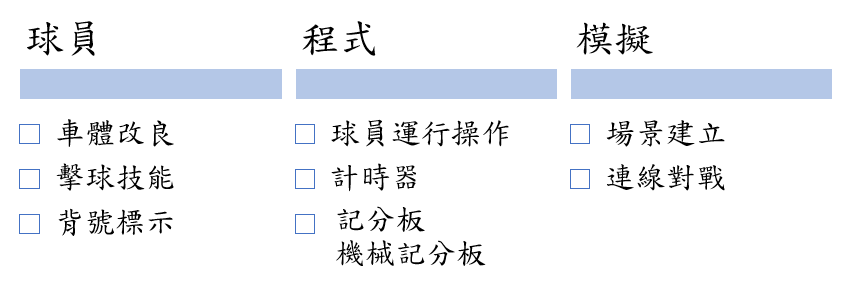
\includegraphics[width=15cm]{35}
\caption{\Large 設計目標圖}\label{fig.35}
\end{center}
\end{figure}
\section{規則說明}\emph{}
類似於足球遊戲,一開始時球會置於場中央,遊戲開始後雙方即可以鍵盤操控機器人,透過防守敵方以及與隊友間的傳球推球至已方的球門得分。\\
遊戲規則如下:
\begin{enumerate}
\item 球觸碰到球門感測器即算得分。
\item 在十分鐘的比賽時間內,獲得最多分數的隊伍即獲勝。
\item 任一方進球得分後,隨機在場內投下新的球,雙方接續進行比賽。
\end{enumerate}

\renewcommand{\baselinestretch}{0.5} %設定行距
%\input{2_machine_learning.tex}
%\input{3_training_env.tex}
%\input{4_simulation.tex}
%\input{5_server.tex}
%=---------------------參考文獻----------------------=%
%\input{9_reference.tex}
%=---------------附錄-----------------=%
\addcontentsline{toc}{chapter}{附錄} %新增目錄名稱
%\input{10_appendix.tex}
\newpage
%=-------------作者簡介-----------------=%
    \addcontentsline{toc}{chapter}{作者簡介}
    \begin{center}
	\fontsize{20pt}{0em}\selectfont \bf{作者簡介}\\
	\end{center}	
	{\begin{textblock}{6}(0,0.5)
	\begin{figure}
	%\includegraphics[width=1.25in]{40923124} 
	\end{figure}
	\end{textblock}
	{\renewcommand\baselinestretch{0.99}\selectfont %設定以下行距
	{\begin{textblock}{15}(3.5,0.7)%{寬度}(以左上角為原點之右移量,下移量)
	\noindent\fontsize{14pt}{0em}\selectfont \makebox[4em][s]{姓名}\enspace:\enspace
    \fontsize{14pt}{0em}\selectfont \makebox[4em][s]{林冠宇}\\     \hspace*{\fill} \\
    \fontsize{14pt}{0em}\selectfont \makebox[4em][s]{學號}\enspace:\enspace
    \fontsize{14pt}{0em}\selectfont \makebox[4em][s]{40923124} \\ %\makebox為文本盒子
    \hspace*{\fill} \\
    \fontsize{14pt}{0em}\selectfont \makebox[4em][s]{就讀學校}\enspace:\enspace
    \fontsize{14pt}{0em}\selectfont \makebox[9em][s]{國立虎尾科技大學}\\
    \fontsize{14pt}{0em}\selectfont \makebox[5em][s]{\quad}\enspace\enspace
    \fontsize{14pt}{0em}\selectfont \makebox[8em][s]{機械設計工程系}\\
    \hspace*{\fill} \\
    \fontsize{14pt}{0em}\selectfont \makebox[4em][s]{經歷}\enspace:\enspace
	\fontsize{14pt}{0em}\selectfont \makebox[9em][s]{國立草屯高級商工職業學校 機械科}\\
    \end{textblock}
	{\begin{textblock}{6}(0,2.3)
	\begin{figure}
	%\includegraphics[width=1.25in]{40923136} 
	\end{figure}
	\end{textblock}
	{\renewcommand\baselinestretch{0.99}\selectfont %設定以下行距
	{\begin{textblock}{15}(3.5,2.5)%{寬度}(以左上角為原點之右移量,下移量)
	\noindent\fontsize{14pt}{0em}\selectfont \makebox[4em][s]{姓名}\enspace:\enspace
    \fontsize{14pt}{0em}\selectfont \makebox[4em][s]{洪士哲}\\     \hspace*{\fill} \\
    \fontsize{14pt}{0em}\selectfont \makebox[4em][s]{學號}\enspace:\enspace
    \fontsize{14pt}{0em}\selectfont \makebox[4em][s]{40923136} \\ %\makebox為文本盒子
    \hspace*{\fill} \\
    \fontsize{14pt}{0em}\selectfont \makebox[4em][s]{就讀學校}\enspace:\enspace
    \fontsize{14pt}{0em}\selectfont \makebox[9em][s]{國立虎尾科技大學}\\
    \fontsize{14pt}{0em}\selectfont \makebox[5em][s]{\quad}\enspace\enspace
    \fontsize{14pt}{0em}\selectfont \makebox[8em][s]{機械設計工程系}\\
    \hspace*{\fill} \\
    \fontsize{14pt}{0em}\selectfont \makebox[4em][s]{經歷}\enspace:\enspace
	 \fontsize{14pt}{0em}\selectfont \makebox[9em][s]{新竹市私立光復高級中學 汽車科}\\
    \end{textblock}
\newpage
%=----------------書背----------------------=%
\pagestyle{empty}%設定沒有頁眉和頁腳
\begin{center}
\fontsize{0.001pt}{1pt}\selectfont .\\
\vspace{4em}
\fontsize{30pt}{30pt}\selectfont 【13】 \\
\fontsize{20pt}{20pt}\selectfont
\vspace{0.5em}
分\\
類\\
編\\
號\\
\vspace{0.5em}
\hspace{-0.5em}:\\
\vspace{0.5em}
\rotatebox[origin=cc]{270}{\sectionef\LARGE \textbf{112-4-APP-3004-1}}\\ %旋轉
\vspace{0.5em}
S\\
o\\
l\\
i\\
d\\
E\\
d\\
g\\
e\\ 
與\\
F\\
e\\
m\\
a\\
p\\
在\\
機\\
械\\
設\\
計\\
上\\
的\\
應\\
用\\
\vspace{2em}
一\\
一\\
三\\
級\\

\end{center}
%\newpage
%\begin{landscape}  %橫式環境
%\begin{center}
%\fontsize{0.001pt}{1pt}\selectfont .
%\vspace{70mm}
%\rotatebox[origin=cc]{90}{\LARGE 【14】}\rotatebox[origin=cc]%{180}{\LARGE 1-2-APP-8765} %旋轉
%\end{center}
%\end{landscape}
\end{document}
